\documentclass{article}

\usepackage{amsmath}
\usepackage{graphicx}

\begin{document}
\title{APMA 4301: Problem Set 4}
\author{Brian Dawes}
\maketitle

\section*{1.}
\subsection*{(a)}
\subsubsection*{i.}
The two elements, $e_1$ and $e_2$, will have the same Mass Matrix due to the symmetry of the problem. Additionally both diagonal terms will be he same as will the two off-diagonal terms. Thus we only need to evaluate two entries to find the Mass Matrices. The diagonal terms are:
\begin{align}
\int_{e_i}\phi_i^2\,dx &=\int_0^\frac 1 2 (1-2x)^2\,dx \nonumber\\
&= \int_0^\frac 1 2 (4x^2-4x+1)\,dx=\frac{4x^3}3-2x^2+x\Big|_0^\frac 1 2 = \frac 1 6
\end{align}

The off-diagonal terms are:
\begin{align}
\int_{e_i}\phi_i\phi_{i+1}\,dx &=\int_0^\frac 1 2 (1-2x)2x\,dx \nonumber\\
&= \int_0^\frac 1 2 (-4x^2+2x)\,dx = -\frac{4x^3}3+x^2 \Big|_0^\frac 1 2 = \frac 1{12}
\end{align}

The overall mass matrix for each element is thus:
\begin{equation}
\boxed{M_{e_i}=
\begin{bmatrix}
\frac 1 6 & \frac 1{12} \\[1ex]
\frac 1{12} & \frac 1 6
\end{bmatrix}
}
\end{equation}

Let $\vec f^{(1)}$ and $\vec f^{(2)}$ be the element forcing vectors for $e_1$ and $e_2$. $\vec b^{(1)}$ can be calculated as:
\begin{align}
f^{(1)}_1&=\int_{e_1} f\phi_1\,dx=\int_0^\frac{1}{2} x(1-x)(1-2x)/2\,dx \nonumber\\
&=\int_0^\frac{1}{2} \left(x^3-\frac{3x^2}2+\frac x 2\right)\,dx=\frac{x^4}4-\frac{x^3}2+\frac{x^2}{4}\Big|_0^\frac 12 = \frac{1}{64}
\end{align}
\begin{align}
f^{(1)}_2&=\int_{e_1} f\phi_2\,dx=\int_0^\frac{1}{2} x(1-x)x\,dx \nonumber\\
&=\int_0^\frac{1}{2} \left(-x^3+\frac x 2\right)\,dx=-\frac{x^4}4-\frac{x^3}3\Big|_0^\frac 12 = \frac{5}{192}
\end{align}

$\vec f^{(2)}$ will simply be $\vec f^{(1)}$ but with the values in reverse order due to the symmetry of the problem. So our element forcing vectors are:
\begin{equation}
\boxed{
\vec f^{(1)}=
\begin{bmatrix}
\frac{1}{64} \\[1ex] \frac{5}{192}
\end{bmatrix},
\quad 
\vec f^{(2)}=
\begin{bmatrix}
\frac{5}{192} \\[1ex] \frac{1}{64}
\end{bmatrix}
}
\end{equation}

\subsubsection*{ii.}
The Mass Matrix for the entire system is:
\begin{equation}
\boxed{
M=
\begin{bmatrix}
\frac{1}{6} & \frac{1}{12} & 0 \\[1ex]
\frac{1}{12} & \frac{1}{3} & \frac{1}{12} \\[1ex]
0 & \frac{1}{12} & \frac{1}{6}
\end{bmatrix}
}
\end{equation}
and the element forcing vector for the system is:
\begin{equation}
\boxed{
\vec f =
\begin{bmatrix}
\frac{1}{64} \\[1ex] \frac{5}{96} \\[1ex] \frac{1}{64}
\end{bmatrix}
}
\end{equation}

\subsubsection*{iii.}
\begin{equation}
M\vec w=\vec f \implies \vec w = M^{-1} \vec f
\end{equation}
\begin{equation}
M^{-1} = 
\begin{bmatrix}
7 & -2 & 1 \\
-2 & 4 & -2 \\
1 & -2 & 7
\end{bmatrix}
\end{equation}
\begin{equation}
\vec w =M^{-1}\vec f=
\boxed{
\begin{bmatrix}
\frac{1}{48} \\[1ex] \frac{7}{48} \\[1ex] \frac{1}{48}
\end{bmatrix}
}
\end{equation}

\subsubsection*{iv.}
\begin{equation}
||e||_{L2}=\left[\int_0^1(\tilde f-f)^2dx\right]^{1/2}
\end{equation}

Since the integrand is symmetric we only have to find the integral from 0 to $\frac{1}{2}$ and double it. In this interval, we have $\tilde f=\frac{1}{48}(14x+1-2x)=\frac{1}{48}(12x+1)$.

So now:
\begin{equation}
||e||_{L2}=\left(2\int_0^{\frac{1}{2}}\left[\frac{1}{48}(12x+1)-x(1-x)/2\right]^2dx\right)^{1/2}\approx 0.0093
\end{equation}

\subsection*{(b)}
Since the problem is quadratic, we will be able to exactly represent it with a quadratic P2. We can find the Galerkin projection then by matching the function at 3 points. We see $f(0)=f(1)=0$ and $f(\frac{1}{2})=\frac{1}{8}$ so our projection should be $\tilde f=0N_1+\frac{1}{8}N_2+0N_3$ as $N_i$ is 1 on the $i$-th point and 0 elsewhere. We see that this gives us $\tilde f=f$ exactly! This also implies that our L2-error is 0 as the integrand is always 0.

\subsection*{(c)}
First, we can easily see that the analytic solution to this problem is:
\begin{equation}
u=\frac{-x^2+3x}{2}
\end{equation}

Now we can solve using the Galerkin projection for the P1 element case.
\begin{equation}
\int vr=\int v\left(\frac{d^2u}{dx^2}-f\right)dx=0
\end{equation}
\begin{equation}
\int v\frac{d^2u}{dx^2}dx = \int vfdx
\end{equation}
\begin{equation}
\int \frac{du}{dx}\frac{dv}{dx}dx+v\frac{du}{dx}|_{\partial\Omega}=\int vfdx
\end{equation}

Now substitute $u=\sum_j w_j\phi_j$, $v=\phi_i$ and switch the sum and integral:
\begin{equation}
\sum_j w_j\int \frac{d\phi_j}{dx}\frac{d\phi_i}{dx}dx=\int\phi_ifdx
\end{equation}
\begin{equation}
a\vec w=\vec f
\end{equation}

We can find $a$ by looking at the contribution of each element. Once again, this will be symmetric so we can just look at the first element:
\begin{equation}
a_{11}=\int_0^{\frac{1}{2}} -2(-2)dx=2
\end{equation}
\begin{equation}
a_{21}=\int_0^{\frac{1}{2}} -2(2d)x=-2
\end{equation}

So the overall matrix is:
\begin{equation}
a=\begin{bmatrix}
2 & -2 & 0 \\
-2 & 4 & -2 \\
0 & -2 & 2
\end{bmatrix}
\end{equation}

Our $\vec f$ can be simply solved for geometrically as $f$ is 1 so they are simply the areas of the basis functions: 
\begin{equation}
\vec f =
\begin{bmatrix}
\frac{1}{4} \\[1ex] \frac{1}{2} \\[1ex] \frac{1}{4}
\end{bmatrix}
\end{equation}

Due to our boundary conditions, we already know 2 values of $\vec w$:
\begin{equation}
\vec w=
\begin{bmatrix}
0 \\ w_2 \\ 1
\end{bmatrix}
\end{equation}

Therefore the only constraint is from the middle row of $a$:
\begin{equation}
0+4w_2-2=\frac{1}{2} \implies w_2=\frac{5}{8}
\end{equation}

So now we can calculate the error:
\begin{align}
||e||_{L2}&=\Big(\int_0^{\frac{1}{2}}\left[\frac{5x}{4}-\frac{-x^2+3x}{2}\right]^2dx \nonumber \\
&+\int_{\frac{1}{2}}^1\left[ 2x-1+\frac{5x}{4}-\frac{-x^2+3x}{2}\right]^2dx\Big)^{1/2}\approx 0.091
\end{align}

For the P2 case, we are once again trying to represent a quadratic function with a quadratic basis so our projection will be exact and we will have 0 error.
\section*{2.}
\subsection*{(a)}
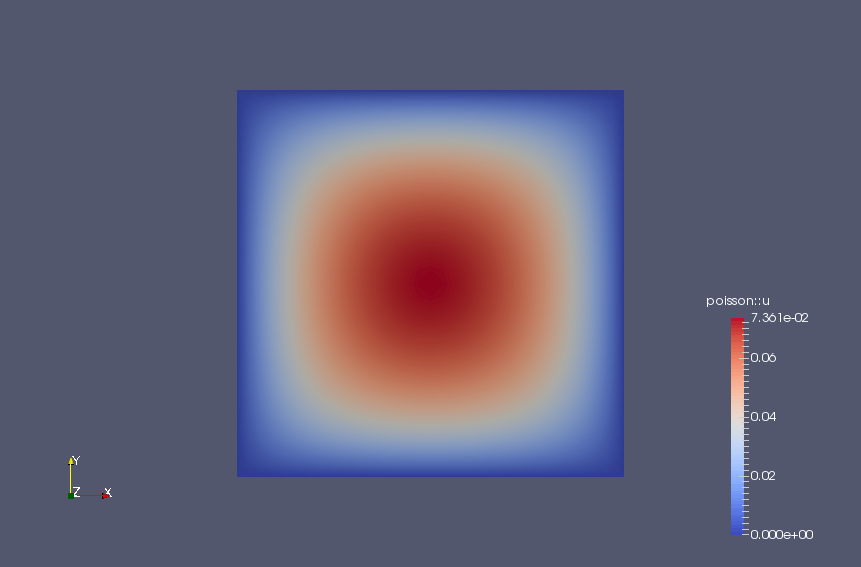
\includegraphics[width=\linewidth]{2a.png}

This image shows the solution to the problem generated by \verb|2a/poisson.tfml|.

\subsection*{(b)}
\subsubsection*{i.}
To change this program I simply modified the mesh geometry to be a rectangle with the given dimensions in the \verb|tfml| file. The spud path in the \verb|shml| file also needed to be modified to a rectangular mesh.

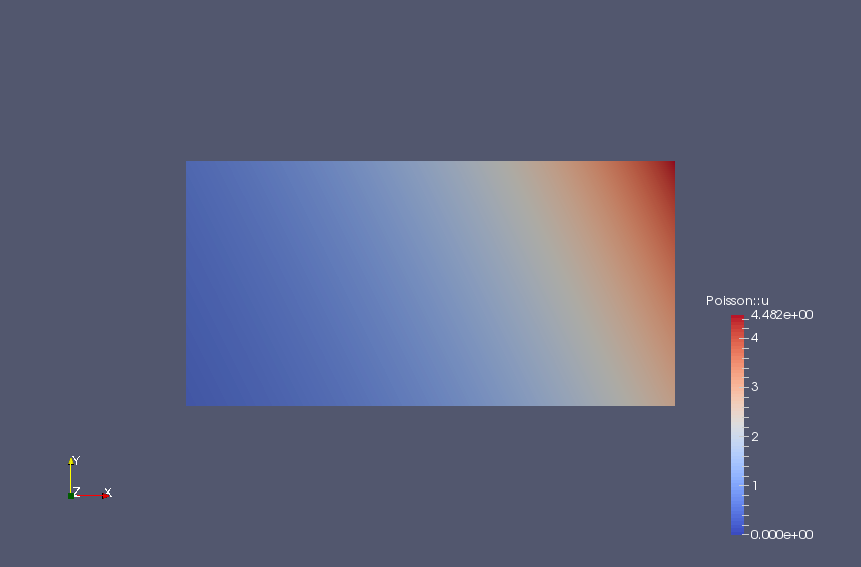
\includegraphics[width=\linewidth]{2biSolution.png}

This image shows the solution to the problem on the rectangle generated by \verb|2bi/poisson.tfml|.

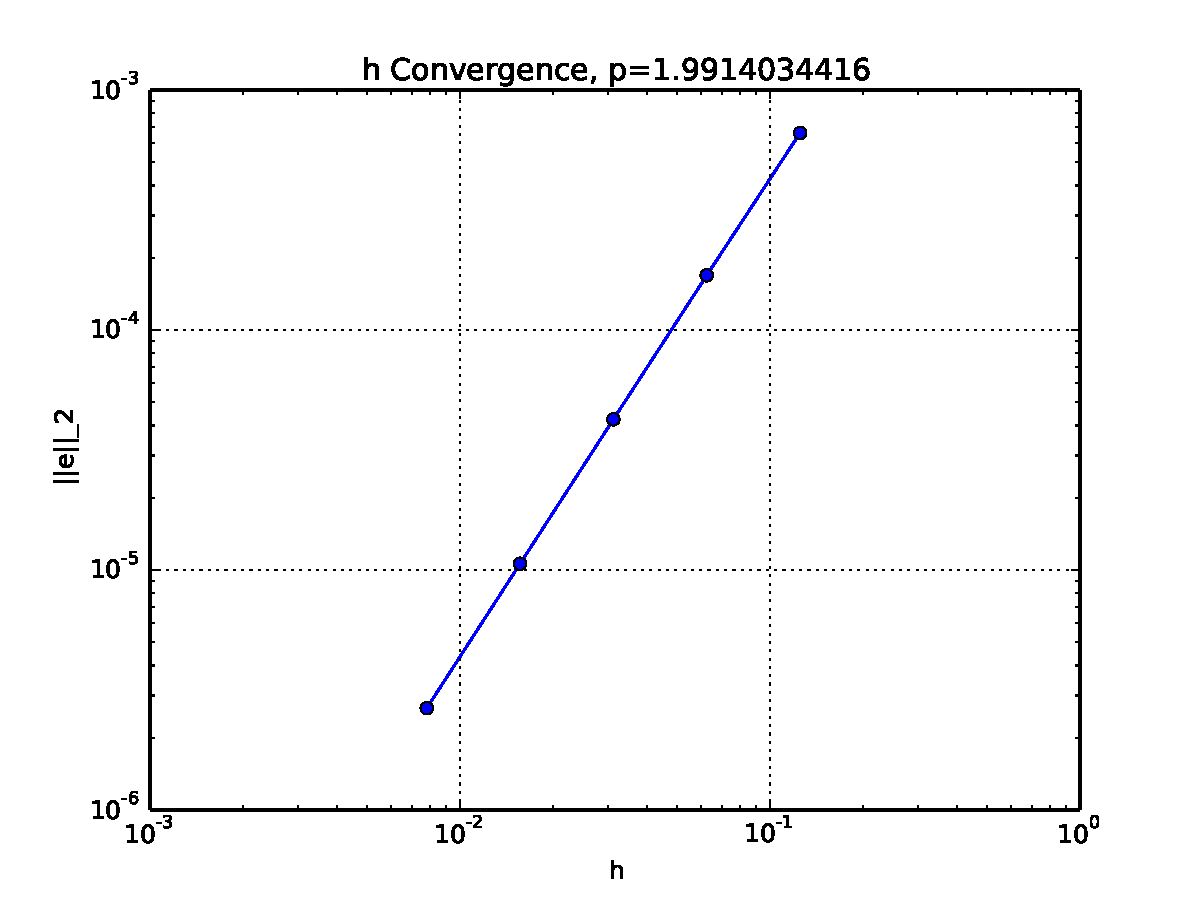
\includegraphics[width=.5\linewidth]{2biConvergence.pdf}
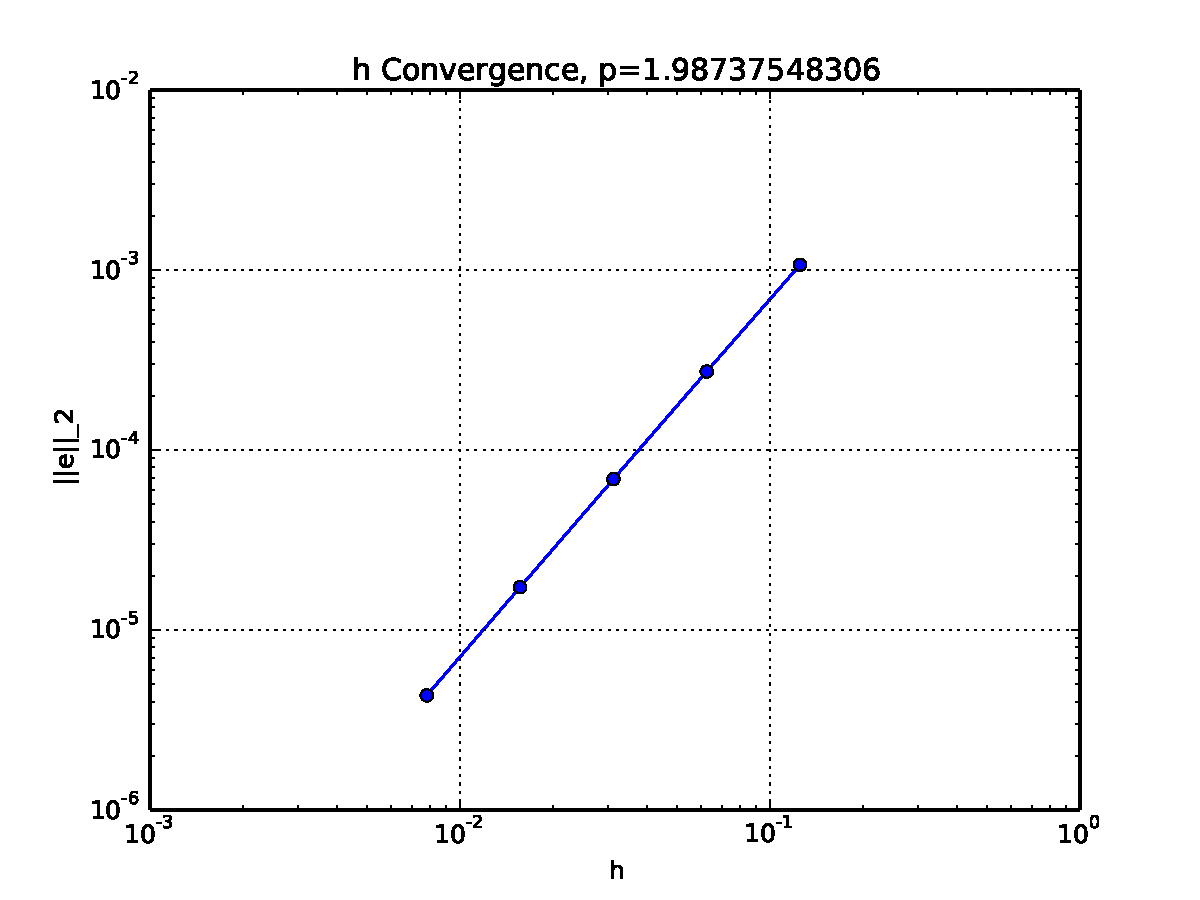
\includegraphics[width=.5\linewidth]{2biConvergenceSquare.pdf}

The left plot shows the convergence on the rectangle and was generated by \verb|2bi/poisson_mms.shml|. The right plot shows the convergence on the unit square and was generated by the \verb|poisson_mms.shml| file contained in the class src repository.

From these two images, we see that both problems converge approximately at the same rate with $p=1.99$. However, for each $h$ value, the error on the unit square is slightly larger. This is because the rectangle has twice the area of the unit square and thus for each $h$ value it has twice as many degrees of freedom and thus has a smaller error.

\subsubsection*{ii.}
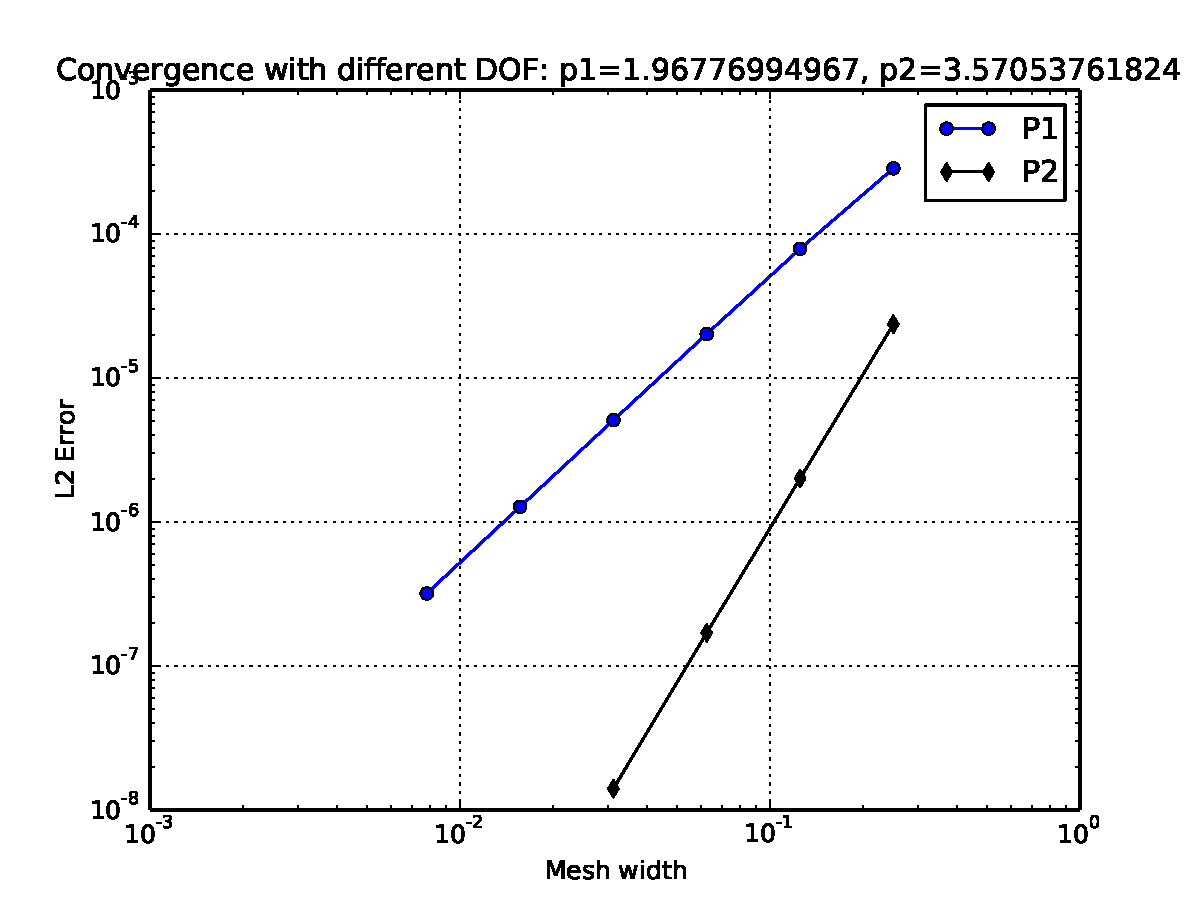
\includegraphics[width=\linewidth]{2biiConvergence.pdf}

This image shows the convergence of the solution with P1 and P2 elements. We see that the P2 elements converge much more rapidly as a function of $h$.

For P1 elements, the error falls below $1e-6$ around $h=4e-3$ which corresponds to 62500 elements. With P2 elements, we need only $h=5e-2$ which corresponds to 400 elements. For P1 elements, there is roughly 1 degree of freedom per element so we have 62500. However for P2 elements, there are roughly 2 degrees of freedom per element so there are about 800 degrees of freedom. The $h=\frac{1}{128}$ P1 case has a wall-time of 4.96 while the $h=\frac{1}{16}$ P2 case has a wall-time of 6.91 and both have approximately the same error. This indicates that simply decreasing $h$ is quicker than increasing $p$.

\subsubsection*{iii.}

I did the second option for this problem. My domain was bounded by the points (1,0), (0,1), (-1,0), and (0,-1) connected by quarter circles and contained a circular hole at the origin with radius $\frac{1}{4}$. This mesh is described by the file \verb|2biii/star.geo| and is run by \verb|2biii/poisson.tfml|. The output is shown in the image below.

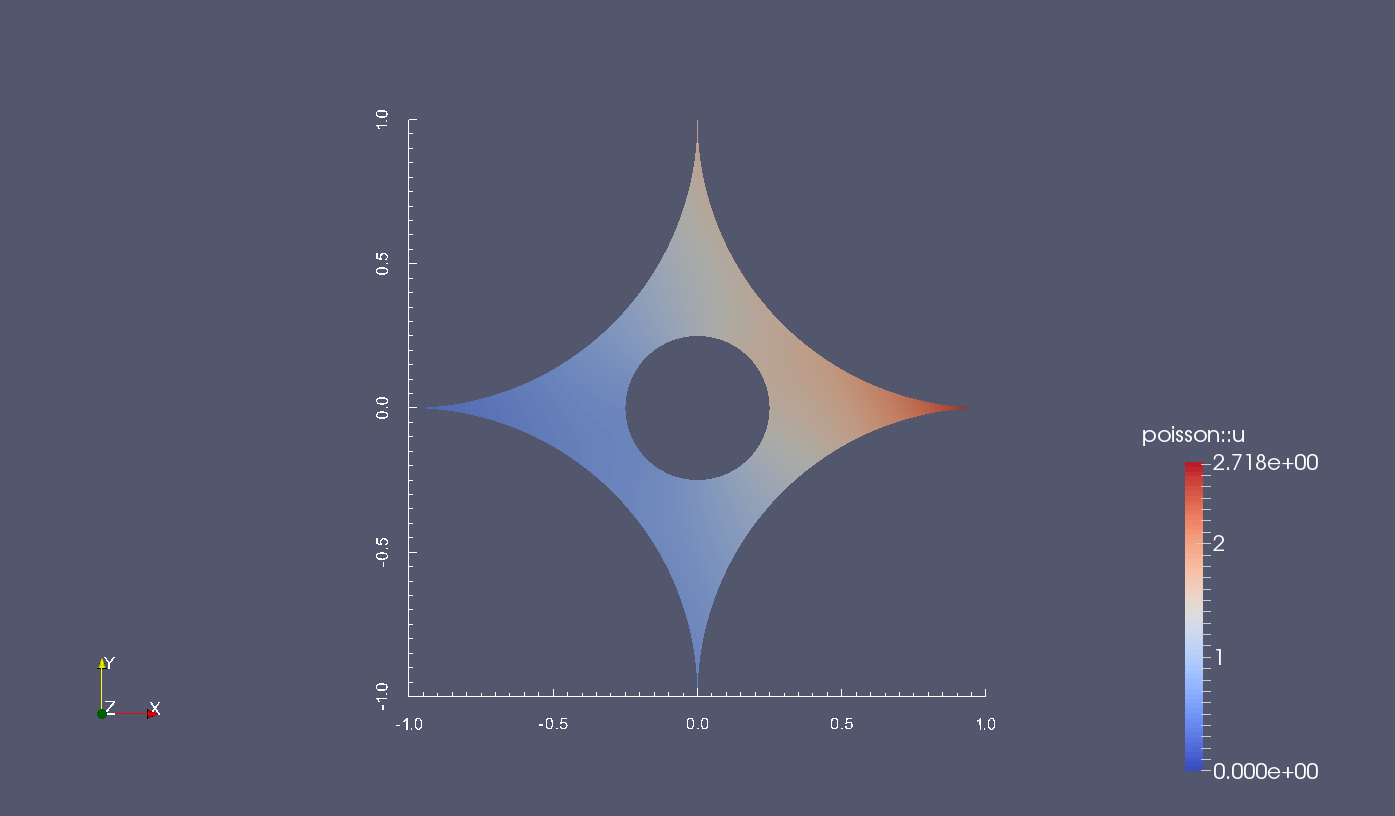
\includegraphics[width=\linewidth]{2biii.png}
\end{document}